% Paquets généraux
\documentclass[a4paper,12pt,titlepage,twoside]{article}
\usepackage[T1]{fontenc}
\usepackage[utf8]{inputenc}
\usepackage[french]{babel}
\usepackage{subcaption}
\addto\captionsfrench{%
  \renewcommand{\tablename}{Tableau}%
}
\usepackage[gen]{eurosym}
%\usepackage[dvips]{graphicx}
\usepackage{minted}
\usepackage{fancyhdr}
\usepackage{pdfpages} 
\usepackage{multido}
\usepackage{hyperref}
\usepackage{textcomp}
\usepackage{schemabloc}
%\usepackage[bitstream-charter]{mathdesign}
\usepackage{array}
\newcolumntype{P}[1]{>{\centering\arraybackslash}p{#1}}
\usepackage[shortlabels]{enumitem}
\usepackage[framemethod=TikZ]{mdframed}

\newcommand{\id}{71}
\newcommand{\nom}{Théorie des mécanismes}
\newcommand{\sequence}{04}
\newcommand{\nomsequence}{Liaisons entre les solides}
\newcommand{\num}{02}
\newcommand{\type}{KH}
\newcommand{\descrip}{Liaisons équivalentes, hyperstatisme, liaisons en série et en parallèle, théorie des graphes}
\newcommand{\competences}{B2-12: Proposer une modélisation des liaisons avec leurs caractéristiques géométriques. \\ &  B2-13: Proposer un modèle cinématique paramétré à partir d'un système réel, d'une maquette numérique ou d'u \\ &  B2-17: Simplifier un modèle de mécanisme. \\ &  B2-18: Modifier un modèle pour le rendre isostatique. \\ &  C1-04: Proposer une démarche permettant d'obtenir une loi entrée-sortie géométrique.  \\ &  C2-05: Caractériser le mouvement d'un repère par rapport à un autre repère. \\ &  C2-06: Déterminer les relations entre les grandeurs géométriques ou cinématiques. }
\newcommand{\nbcomp}{7}
\newcommand{\systemes}{}
\newcommand{\systemesnum}{}
\newcommand{\systemessansaccent}{}
\newcommand{\ilot}{2}
\newcommand{\ilotstr}{02}
\newcommand{\dossierilot}{\detokenize{Ilot_02 }}

%\usepackage{style}
\usepackage{bodegraph}
\usepackage{rpcinematik}
\usepackage[locale = FR]{siunitx}
\usepackage{caption}
\newcommand{\institute}{Lycée Dorian}

\usepackage{listings}
\usepackage{fancyvrb}
\usepackage{color}
\usepackage{xcolor}
\usepackage{colortbl}
\usepackage{helvet}
\usepackage[frenchmath]{newtxsf} % for sans serif symbols
\renewcommand{\familydefault}{\sfdefault}
%\usepackage{amsfonts}
%\usepackage{amsmath}
%\usepackage{lmodern}
\usepackage{mathastext}
%\usepackage{xspace}
\usepackage{varioref}
\usepackage{tabularx}
%\usepackage{floatflt}
\usepackage{graphics}
\usepackage{wrapfig}
\usepackage{textcomp}
\usepackage{tikz,tkz-tab}
\usepackage[european resistor, european voltage, european current]{circuitikz}
\usepackage{wrapfig}
\usepackage{gensymb}
\usepackage[percent]{overpic}
\usetikzlibrary{babel}
\usepackage{ifthen}
\usepackage{cancel}
\usepackage{etoolbox}
\usepackage{multirow}
%\usepackage{boxedminipage}
\definecolor{gris25}{gray}{0.75}
\definecolor{bleu}{RGB}{18,33,98}
\definecolor{bleuf}{RGB}{42,94,171}
\definecolor{bleuc}{RGB}{231,239,247}
\definecolor{bleum}{RGB}{160,195,226}
\definecolor{rougef}{RGB}{185,18,27}
\definecolor{rougec}{RGB}{255,188,204}%255,230,231
\definecolor{vertf}{RGB}{103,126,82}
\definecolor{vertc}{RGB}{220,255,191}
\definecolor{forestgreen}{rgb}{0.13,0.54,0.13}
\definecolor{blcr}{rgb}{0.59,0.69,0.84}
\definecolor{blfr}{rgb}{0.32,0.51,0.75}
\definecolor{orfr}{rgb}{0.90,0.42,0.15}
\definecolor{orcr}{rgb}{0.90,0.65,0.50}
\definecolor{orangef}{rgb}{0.659,0.269,0.072}
\definecolor{orange}{rgb}{0.58,0.35,0.063}
\definecolor{orangec}{rgb}{0.43,0.32,0.25}
\definecolor{rcorrect}{rgb}{0.6,0,0}
\definecolor{sequence}{rgb}{0.75,0.75,0.75}
\definecolor{competences}{rgb}{0.61,0.73,0.35}
\definecolor{rose}{HTML}{ff00ff}
\definecolor{grisf}{HTML}{222222}
\definecolor{grisc}{HTML}{636363}
\definecolor{normal}{HTML}{4087c4}
\definecolor{info}{HTML}{5bc0de}
\definecolor{success}{RGB}{92,184,92}
\definecolor{warning}{RGB}{240,173,78}
\definecolor{danger}{RGB}{217,83,79}
\hypersetup{                    % parametrage des hyperliens
    colorlinks=true,                % colorise les liens
    breaklinks=true,                % permet les retours à la ligne pour les liens trop longs
    urlcolor= blfr,                 % couleur des hyperliens
    linkcolor= orange,                % couleur des liens internes aux documents (index, figures, tableaux, equations,...)
    citecolor= forestgreen                % couleur des liens vers les references bibliographiques
    }

\newcolumntype{M}[1]{>{\centering\arraybackslash}m{#1}}
\definecolor{codegreen}{rgb}{0,0.6,0}
\definecolor{codegray}{rgb}{0.5,0.5,0.5}
\definecolor{codepurple}{rgb}{0.58,0,0.82}
\definecolor{backcolour}{rgb}{0.95,0.95,0.92}

\lstdefinestyle{mystyle}{
    backgroundcolor=\color{backcolour},   
    commentstyle=\color{codegreen},
    keywordstyle=\color{magenta},
    numberstyle=\tiny\color{codegray},
    stringstyle=\color{codepurple},
    basicstyle=\ttfamily\footnotesize,
    breakatwhitespace=false,         
    breaklines=true,                 
    captionpos=b,                    
    keepspaces=true,                 
    numbers=left,                    
    numbersep=5pt,                  
    showspaces=false,                
    showstringspaces=false,
    showtabs=false,                  
    tabsize=2
}

\lstset{style=mystyle}

% Mise en page
\pagestyle{fancy}

\setlength{\hoffset}{-18pt}
\setlength{\oddsidemargin}{0pt} 	% Marge gauche sur pages impaire2s
\setlength{\evensidemargin}{0pt} 	% Marge gauche sur pages paires
\setlength{\marginparwidth}{00pt} 	% Largeur de note dans la marge
\setlength{\headwidth}{481pt} 	 	% Largeur de la zone de tête (17cm)
\setlength{\textwidth}{481pt} 	 	% Largeu\textbf{r de la zone de texte (17cm)
\setlength{\voffset}{-18pt} 		% Bon pour DOS
\setlength{\marginparsep}{7pt}	 	% Séparation de la marge
\setlength{\topmargin}{-30pt} 		% Pas de marge en haut
\setlength{\headheight}{55pt} 		% Haut de page
\setlength{\headsep}{20pt} 		% Entre le haut de page et le texte
\setlength{\footskip}{30pt} 		% Bas de\textbf{ page + séparation
\setlength{\textheight}{700pt} 		% Hauteur de l'icone zone de texte (25cm)
\setlength\fboxrule{1 pt}
\renewcommand{\baselinestretch}{1}
\setcounter{tocdepth}{1}
\newcommand{\cadre}[2]
{\fbox{
  \begin{minipage}{#1\linewidth}
   \begin{center}
    #2\\
   \end{center}
  \end{minipage}
 }
}

\newcommand{\repon}[1]
{
~\ \\
\begin{tabular}{|m{\linewidth}|}
 \hline
\multido{}{#1}{\\ \hline}
\end{tabular}
}


\newcommand{\objectif}[1]{
\mdfsetup{%
frametitle={%
\tikz[baseline=(current bounding box.east),outer sep=0pt]
\node[anchor=east,rectangle,fill=bleum]
{\strut Objectif~};}}
\mdfsetup{innertopmargin=10pt,linecolor=bleum,%
linewidth=2pt,topline=true,%
frametitleaboveskip=\dimexpr-\ht\strutbox\relax
}
\begin{mdframed}[]\relax%
#1
\end{mdframed}}


\newcounter{num_quest} \setcounter{num_quest}{0}
\newcounter{num_rep} \setcounter{num_rep}{0}
\newcounter{num_cor} \setcounter{num_cor}{0}

\newcommand{\feuilleDR}[1]{
	\begin{tikzpicture}
		\draw[gray!30](0,0)grid[step=0.5cm](\linewidth,#1);
	\end{tikzpicture}
}

%\newcommand{\question}[1]{\refstepcounter{num_quest}\par
%~\ \\ \parbox[t][][t]{0.15\linewidth}{\textbf{Question \arabic{num_quest}}}\parbox[t][][t]{0.85\linewidth}{#1\label{q\the\value{num_quest}}}\par
%}

\newcommand{\question}[1]{\refstepcounter{num_quest}\par
~\ \\ \textbf{Question \arabic{num_quest} : }#1\label{q\the\value{num_quest}}\par
}

\newcommand{\posetafigure}[3]{
\begin{figure}[ht!]
 \begin{center}
  \includegraphics[width=#2\linewidth]{img/#1}
 \end{center}
 \caption{\label{#1} #3}
\end{figure}}

\newcommand{\goforum}{
\begin{figure}

\end{figure}
\begin{center}
 
\includegraphics[width=0.7\linewidth]{../../../img/go_forum}
\end{center}
\label{go_forum}
\caption{J'pète les plombs}
\end{figure}}

\newcommand{\reponse}[4][1]
{\noindent
\parbox{\textwidth}{
\rule{\linewidth}{.5pt}\\
\textbf{Question\ifthenelse{#1>1}{s}{} \multido{}{#1}{%
\refstepcounter{num_rep}\ref{q\the\value{num_rep}} }:} ~\ \\
\ifdef{\public}{#3 \ifthenelse{#2>0}{~\ \\ 	\feuilleDR{#2}}}{#4}
}}

\newcommand{\cor}
{\refstepcounter{num_cor}
\noindent
\rule{\linewidth}{.5pt}
\textbf{Question \arabic{num_cor}:} \\
}

\newcommand{\finsujet}
{
    \begin{center}
    \Large{FIN}
    \end{center}

    \cleardoublepage

    \ifdef{\public}{\pagestyle{docreponse}}{\pagestyle{correction}}

    \ifdef{\public}{
        \begin{tikzpicture} 
            \draw (0,0) rectangle (2,2);
            \draw (0,0) -- (2,2);
            \draw (1.5,0.5) node {\large 20};
            \draw (2.5,0) rectangle (16,2);
            \draw (4.5,1.7) node {\large Commentaires:};
        \end{tikzpicture}
    }
    ~\ \\
}


%\newcommand{\repcarre}[2]
%{
%~\ \\
%\begin{tikzpicture}
%\draw [fill=white] (0,0) rectangle +(\linewidth,#1);
%\node[align=left] at (1.1,#2-0.3) {\textbf{Question #1:}};
%\end{tikzpicture}
%}

\newcommand{\titre}[1]
{\begin{center}
\cadre{0.8}{\huge #1} 
\end{center}
}


%Définition des torseurs :
\newcommand{\torseur}[2]{\left\{\mathcal{#1}_{#2} \right\}}
\newcommand{\torseurh}[3]{\left\{\genfrac{}{}{0pt}{0}{#1}{#2}\right\}_{#3}}
\newcommand{\torseurv}[8]{\left\{
\begin{matrix}
#1 & #4 \\ #2 & #5 \\ #3 &#6
\end{matrix}
\right\}_{{#7},{#8}}}

%Définition des torseurs :
%\newcommand{\torseur}[2]{\left \{\mbox{\relsize{2}{$\mathcal {#1}$}\relsize{-2}}\phantom{}_{\mbox{\scriptsize $#2$}} \right \}}
%\newcommand{\torseurh}[3]{\left\{\genfrac{}{}{0pt}{0}{#1}{#2}\right\}_{#3}}
%\newcommand{\torseurv}[8]{
%\left\{\begin{array}{@{}c|c@{}} #1 & #4 \\ #2 & #5 \\ #3 & #6 \end{array} \right\}_{#7,#8}
%}
\newcommand{\derivee}[2]{\left.\dfrac{\d #1}{\d t}\right|_{#2}}
\newcommand{\tripleint}{\int\!\!\!\!\!\int\!\!\!\!\!\int}

% Notation cinématique et statique
\newcommand{\cinematique}[2]{\mbox{#1}/\mbox{#2}}
\newcommand{\statique}[2]{\mbox{#1}\rightarrow\mbox{#2}}
\newcommand{\moment}[3]{\vv {#1}_{\scriptsize{#3}}(#2)}
\newcommand{\resultante}[2]{\vv {#1}_{\scriptsize{#2}}}


%Commande de base
\newcommand{\jo}{\left(j\omega\right)} % j \omega dans l'analyse fréquentielle
\newcommand{\tl}{\xrightarrow{\mathcal{L}}} % transformée de laplace sur fleche
\newcommand{\tli}{\xrightarrow{\mathcal{L}^{-1}}} % transformée inverse de laplace sur fleche
\renewcommand{\d}[1][]{\mathrm{d#1}}
\newcommand{\dd}[1][]{\mathrm{d#1}}
\newcommand{\vect}[2]{{#1}\wedge{#2}}
\newcommand{\base}[3]{(\vec #1,\vec #2,\vec #3)}
\newcommand{\vectbase}[4]{{\vphantom{\left| \begin{matrix}
#1\\#2\\#3 \end{matrix} \right|}}_{#4}{\left| \begin{matrix}
#1\\#2\\#3 \end{matrix} \right.}}
%Pour avoir les paragraphes sous la forme I, II, III
\renewcommand{\thesection}{\Roman{section}}
\setcounter{secnumdepth}{3}
\renewcommand{\Frlabelitemii}{$\bullet$}

% En tête et pied de page
\lhead{\nom}
\rhead{
\includegraphics[width=2cm]{../../../img/logo}}
\lfoot{\auteurun,\ \auteurdeux}
\cfoot{Page \thepage}

\fancypagestyle{docreponse}{%
  \fancyhf{}
  \fancyhead[LO]{NOM Prénom: .............................}
  \rhead{
\includegraphics[width=2cm]{../../../img/logo}\hspace{2pt}}
  \ifdef{\auteurdeux}{\lfoot{\auteurun,\ \auteurdeux}}{\lfoot{\auteurun}}
  \rfoot{\nom}
  \lfoot{Document réponse}
  \cfoot{Page \thepage}
   }

\fancypagestyle{correction}{%
  \fancyhf{}
  \lhead{\colorbox{danger}{\begin{minipage}{0.65\paperwidth} \textcolor{white}{\textbf{Correction}} \end{minipage}} }
  \rhead{
\includegraphics[width=2cm]{../../../img/logo}}
  \lfoot{Renaud Costadoat, Françoise Puig}
  \rfoot{\colorbox{danger}{\begin{minipage}{0.4\paperwidth} \begin{flushright}\textcolor{white}{\textbf{Correction}}\end{flushright} \end{minipage}} }}

\fancypagestyle{correctioninfo}{%
  \fancyhf{}
  \lhead{\colorbox{danger}{\begin{minipage}{0.65\paperwidth} \textcolor{white}{\textbf{Correction}} \end{minipage}} }
  \rhead{
\includegraphics[width=2cm]{../../../img/logo}}
  \lfoot{Renaud Costadoat, Juliette Genzmer}
  \rfoot{\colorbox{danger}{\begin{minipage}{0.6\paperwidth} \begin{flushright}\textcolor{white}{\textbf{Correction}}\end{flushright} \end{minipage}} }}

\renewcommand{\footrulewidth}{0.4pt}

\usepackage{eso-pic}
\newcommand{\BackgroundPic}{%
\put(0,0){%
\parbox[b][\paperheight]{\paperwidth}{%
\vfill
\begin{center}
\hspace{0.5cm}\vspace{0.5cm}

\includegraphics[width=\paperwidth,height=\paperheight,%
keepaspectratio]{../../../img/fond3}%
\end{center}
\vfill
}}}

\newcommand{\BackgroundPicdeux}{%
\put(25,-30){%
\parbox[b][\paperheight]{\paperwidth}{%
\vfill
\begin{center}
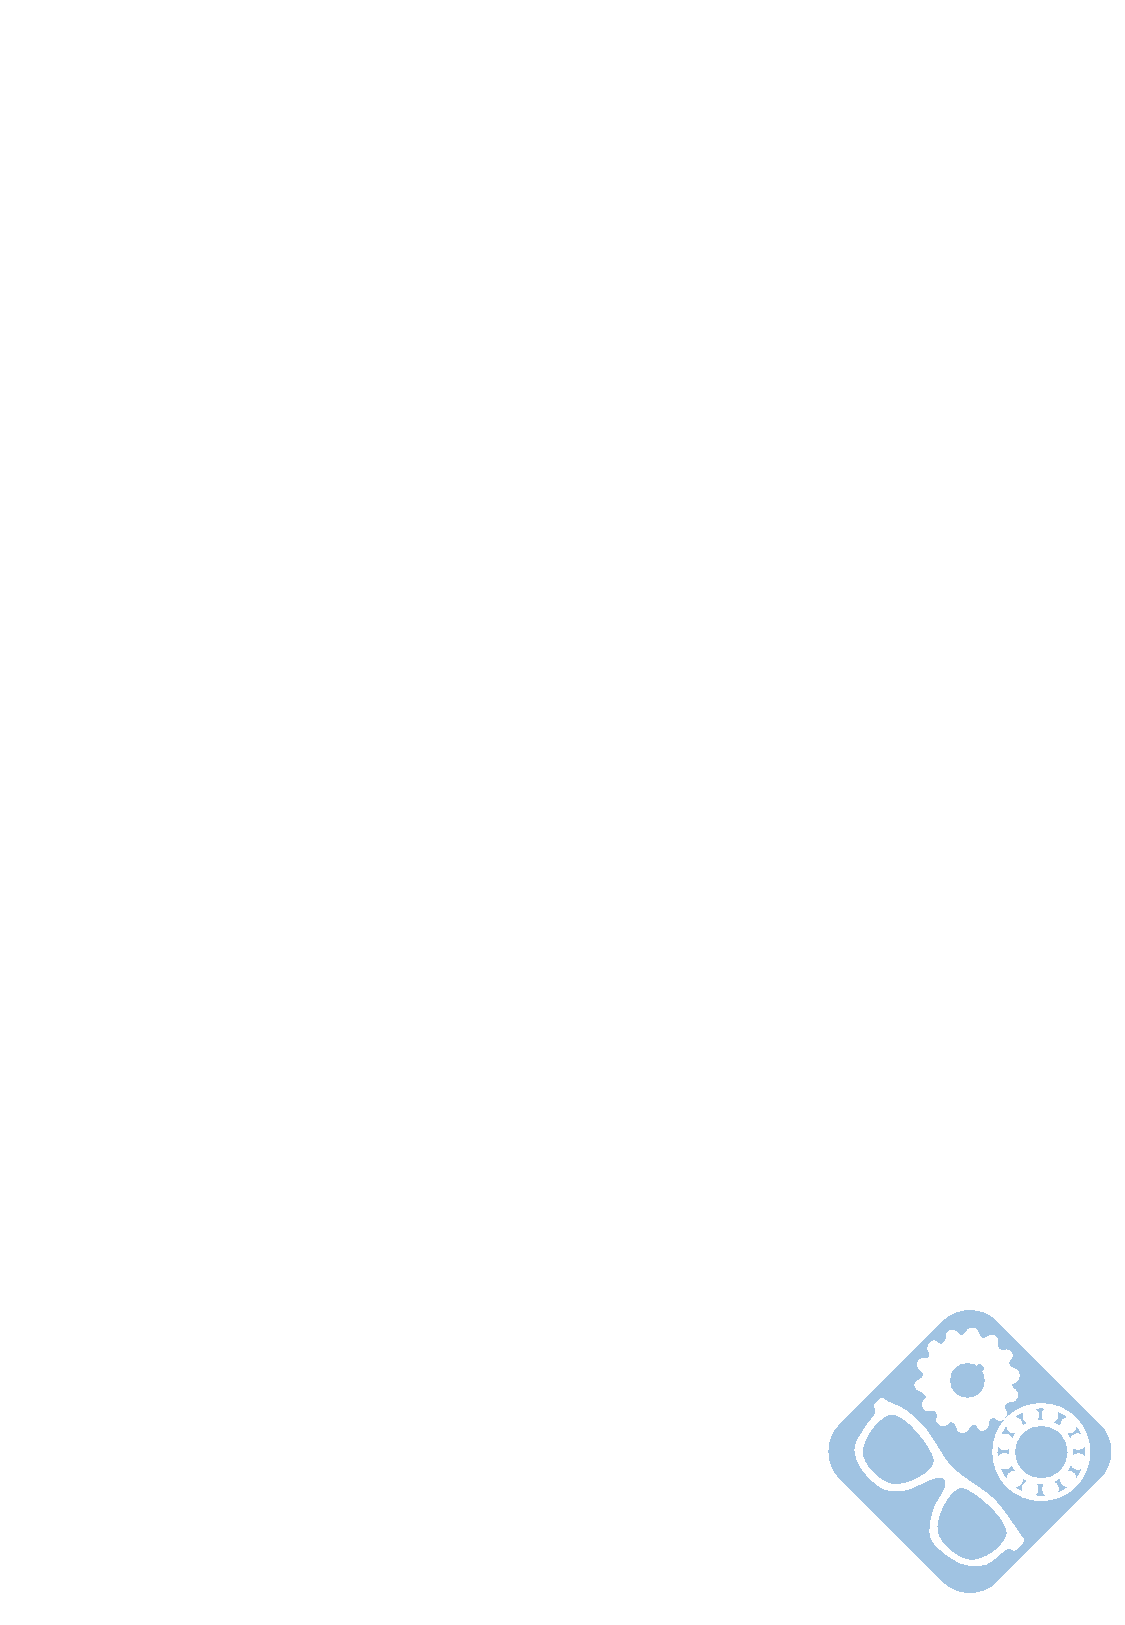
\includegraphics[width=\paperwidth,height=\paperheight,%
keepaspectratio]{../../../img/fond4}%
\end{center}
\vfill
}}}

\begin{document}

\pagestyle{empty}

\AddToShipoutPicture*{\BackgroundPic}


\includegraphics[width=2cm]{../../../img/logo}

\Huge{DS \numero - \sujet}

\vspace{1cm}

\ifdef{\prive}{\begin{center}\colorbox{danger}{\Huge{Avec Correction}}\end{center}}{}

\begin{center}
\centering\huge{PTSI}
\end{center}

\vspace{2cm}


\begin{center}
\centering\Large{\jour}
\end{center}

\vspace{2cm}

\normalsize

\tableofcontents

\newpage

\AddToShipoutPicture{\BackgroundPicdeux}

\pagestyle{fancy}

\begin{center}
\Huge \sujet
\end{center}


\normalsize


\section*{Présentation générale}

\begin{figure}[ht!]
 \begin{minipage}{0.6\linewidth}
 Le système étudié dans ce sujet, appelé Hublex, est un gyropode professionnel destiné à faciliter le déplacement des collaborateurs au sein d'entreprises, administrations, hôpitaux... lorsque ces lieux sont de grandes tailles. La figure 1 montre un exemple d'utilisation dans l'entrepôt d'une entreprise de logistique.

Il est en effet prouvé que les déplacements piétons sur les lieux de travail peuvent générer, s'ils sont répétitifs, des fatigues extrêmes ainsi que des troubles musculosquelettiques. Il n'est pas rare, par exemple, qu'au cours d'une journée, des employés marchent plusieurs kilomètres sur leur lieu de travail, parfois sous la forme de micro-déplacements. C'est dans ce contexte qu'a été conçu, en France, le Hublex.
 \end{minipage}\hfill
 \begin{minipage}{0.35\linewidth}
 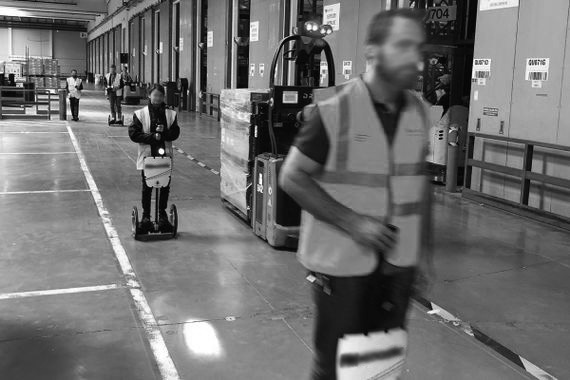
\includegraphics[width=\linewidth]{img/fig01}
 \caption{\label{fig01}Hublex en utilisation dans une entreprise de logistique}
 \end{minipage}
\end{figure}

\begin{figure}[ht!]
 \begin{minipage}{0.7\linewidth}

Ce gyropode doit permettre de réduire la fatigue des collaborateurs afin d'augmenter leur bien-être. Sa particularité est d'avoir été spécifiquement créé pour s'intégrer dans un environnement de travail grâce à des caractéristiques techniques qui le différencient des gyropodes classiques :
\begin{itemize}
 \item Prise en main en moins de 5 minutes,
 \item Maniabilité optimisée,
 \item Faible largeur, inférieure à 40 cm,
 \item Léger, moins de 12 kg,
 \item Utilisable 24 h/24 grâce à sa batterie interchangeable.
\end{itemize}


On peut voir, figure \ref{fig02}, une vue générale du produit. Les principales exigences du système sont présentées dans le diagramme d'exigences de la figure \ref{fig16}.

\paragraph{Description du produit}

Le Hublex se caractérise par une conception originale alliant une structure et une motorisation à la fois épurées mais aussi très modernes (voir figure \ref{fig03}). Le châssis est constitué de pièces évidées et les roues sont sans moyeu (\og hubless \fg en anglais).
 \end{minipage}\hfill
 \begin{minipage}{0.25\linewidth}
 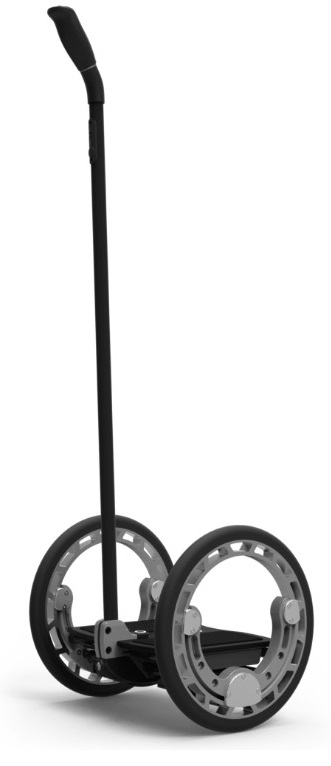
\includegraphics[width=\linewidth]{img/fig02}
 \caption{\label{fig02}Vue générale du Hublex}
 \end{minipage}
\end{figure}

La liaison pivot entre chaque roue et le châssis est astucieusement réalisée par l'intermédiaire de liaisons quasi ponctuelles, ce qui permet de limiter le coût et la quantité de matière nécessaire à sa réalisation.
 
Chaque roue possède sa propre motorisation constituée d'une machine synchrone avec autopilotage permettant de s'affranchir de l'utilisation d'un réducteur. La transmission se résume à un galet directement lié à l'arbre moteur entraînant la roue (voir figure \ref{fig04}).

\begin{figure}[ht!]
 \begin{minipage}{0.45\linewidth}
 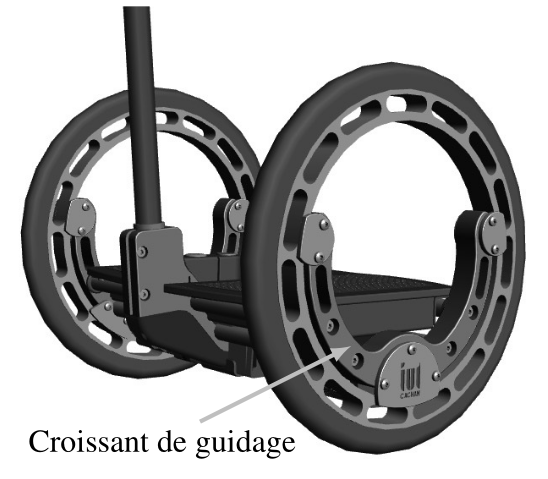
\includegraphics[width=\linewidth]{img/fig03}
 \caption{\label{fig03}Vue extérieure de la structure}
 \end{minipage}\hfill
 \begin{minipage}{0.45\linewidth}
 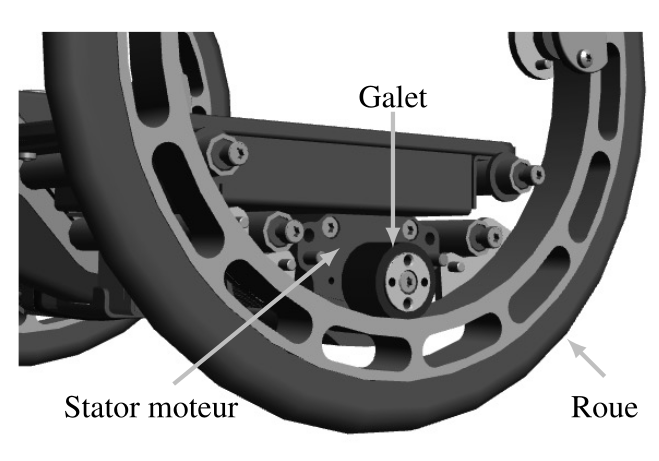
\includegraphics[width=\linewidth]{img/fig04}
 \caption{\label{fig04}Détail de la transmission par galet (sans croissant de guidage)}
 \end{minipage}
\end{figure}

\paragraph{Principe de fonctionnement général}

~\

\begin{figure}[h!]
 \begin{minipage}{0.4\linewidth}
Les principaux composants constituant un Hublex sont rassemblés dans le diagramme de bloc interne
(figure \ref{fig05}).

Le pilote commande la direction et la vitesse. Pour avancer ou reculer, il influe sur l'inclinaison du
châssis du Hublex en se penchant en avant ou en arrière. Cette inclinaison, mesurée grâce à une centrale inertielle, correspond à une consigne d'accélération imposée par le pilote. Lorsqu'il se penche, l'équilibre de l'ensemble {Hublex + pilote} est assuré par le Hublex lui-même grâce à un asservissement visant à le redresser.
 \end{minipage}\hfill
 \begin{minipage}{0.55\linewidth}
 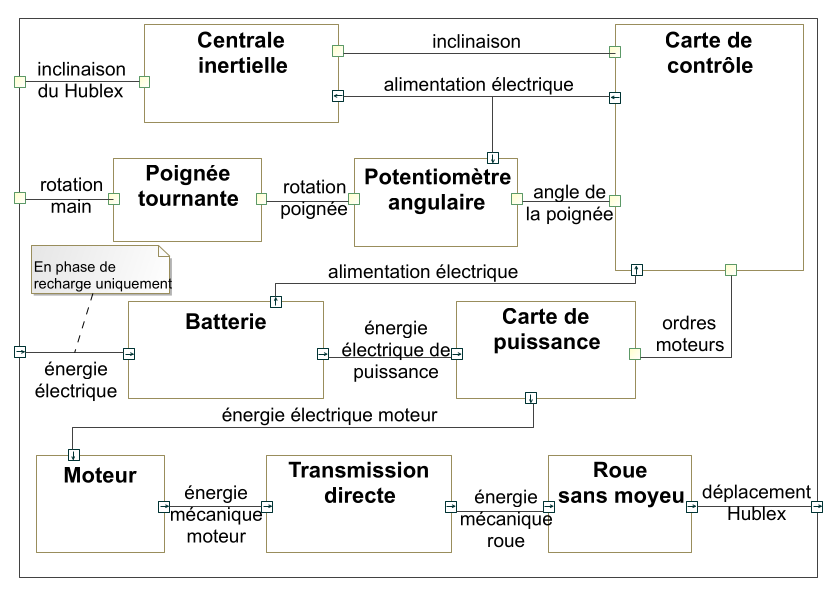
\includegraphics[width=\linewidth]{img/fig05}
 \caption{\label{fig05}Diagramme de bloc interne}
 \end{minipage}
\end{figure}


La trajectoire du Hublex est, quant à elle, imposée par le pilote à l'aide d'une poignée située au bout
du manche qu'il tourne en fonction de la direction souhaitée. Ainsi, la vitesse de chaque moteur est construite à partir de ces deux commandes. C'est la carte de contrôle qui génère la consigne d'intensité
électrique imposée au moteur par l'intermédiaire d'un onduleur situé dans la carte de puissance.

\question{Compléter le schéma fonctionnel du document réponse, en précisant le nom des composants associés aux
fonctions, ainsi que le type de chaque flux (I pour information, E pour énergie, M pour matière). On y reportera uniquement les composants présents dans le diagramme de bloc interne (figure \ref{fig05}).}

\section{Génération de la consigne des vitesses moteurs}

\paragraph{Objectif :} analyser le comportement cinématique du Hublex en virage et sur sol plat, afin d'obtenir la consigne de vitesse à imposer aux moteurs permettant de répondre notamment aux exigences \og 1.1.1 \fg\ et \og 1.4.3 \fg.

\subsection{Paramétrage du Hublex en trajectoire circulaire}

Le Hublex dispose de deux moteurs permettant d'entraîner chaque roue indépendamment l'une de l'autre. Le mode de transmission utilisé est un mode direct par friction, de rapport k = 0.092, entre un galet solidaire de l'arbre moteur gauche \textbf{4} et la jante de la roue gauche \textbf{2} Ainsi, $\omega_{21}=k\cdot\omega_{41}$ et $\omega_{31}=k\cdot\omega_{51}$. La transmission côté droit est identique. Les arbres moteurs gauche \textbf{4} et droit \textbf{5} ne sont pas représentés.

On note $\overrightarrow{V_{M,S_i/R_j}}$ la vitesse du point $M$ dans le mouvement du solide $S_i$ par rapport au repère $R_j$.

Le paramétrage est donné sur les figures \ref{fig06}, \ref{fig07} et \ref{fig08}. On définit :
\begin{itemize}
 \item Le repère $R_0(O_0,\vec{x_0},\vec{y_0},\vec{z_0})$ lié au sol \textbf{0},
 \item Le repère $R_1(O_1,\vec{x_1},\vec{y_1},\vec{z_1})$ lié au châssis \textbf{1} du Hublex, avec $O_1$ le point situé au centre du châssis \textbf{1} et sur l'axe de rotation des roues tel que $\overrightarrow{V_{O_1,S_1/R_0}}= V\cdot \vec{y_1}$,
 \item Le repère $R_2(A,\vec{x_2},\vec{y_2},\vec{z_2})$ lié à la roue gauche \textbf{2}, avec $A$ le centre de la roue gauche,
 \item Le repère $R_3(B,\vec{x_3},\vec{y_3},\vec{z_3})$ lié à la roue droite \textbf{3}, avec $B$ le centre de la roue droite.
\end{itemize}

On note le vecteur constant $\overrightarrow{AB}=L\cdot \vec{x_1}$ et $R$ le rayon d'une roue.

On s'intéresse à une trajectoire du Hublex (châssis \textbf{1}) par rapport au sol de type circulaire, de centre
$O_0$ et de rayon de courbure $r_c$, telle que définie figure \ref{fig08}. Les roues sont en contact avec le sol au point $I$ (pour la roue gauche \textbf{2}) et au point $J$ (pour la roue droite \textbf{3}). On fera l'hypothèse de roulement sans glissement des roues sur le sol en ces points. Le graphe des liaisons associé est donné figure \ref{fig09}.

On définit :
\begin{itemize}
 \item La position angulaire du châssis \textbf{1} par rapport au sol \textbf{0} par l'angle $\theta_{10}$, autour de $\vec{z_0}= \vec{z_1}$ tel que $\theta_{10}=(\vec{x_0},\vec{x_1})=(\vec{y_0},\vec{y_1})$,
 \item La position angulaire de la roue gauche \textbf{2} par rapport au châssis \textbf{1} par l'angle $\theta_{21}$, autour de $\vec{x_1}=\vec{x_2}$ tel que $\theta_{21}=(\vec{y_1},\vec{y_2})=(\vec{z_1},\vec{z_2})$,
 \item La position angulaire de la roue droite \textbf{3} par rapport au châssis \textbf{1} par l'angle $\theta_{31}$, autour de $\vec{x_1}=\vec{x_3}$ tel que $\theta_{31}=(\vec{y_1},\vec{y_3})=(\vec{z_1},\vec{z_3})$.
\end{itemize}

\newpage

On note :
\begin{itemize}
 \item Les vitesses angulaires associées : $\omega_{10}=\dfrac{d\theta_{10}}{dt}$,$\omega_{21}=\dfrac{d\theta_{21}}{dt}$,$\omega_{31}=\dfrac{d\theta_{31}}{dt}$,
 \item La vitesse de rotation de l'arbre moteur gauche \textbf{4} (respectivement arbre moteur droit \textbf{5}), non représenté sur les figures, par rapport au châssis \textbf{1} par $\omega_{41}$ (respectivement $\omega_{51}$).
\end{itemize}

\subsection{Étude de la cinématique pour une trajectoire circulaire}

\question{A partir de la figure \ref{fig08}, écrire $\overrightarrow{O_0O_1}$ dans la base $R_1$.

Déterminer $\overrightarrow{V_{O_1,S_1/R_0}}=\left[\dfrac{d\overrightarrow{O_0O_1}}{dt}\right]_{R_0}$.En déduire la relation entre $V$, $r_c$ et $\omega_{10}$.}

\question{En utilisant l'hypothèse de roulement sans glissement $\left(\overrightarrow{V_{I,S_2/R_0}}\ et\ \overrightarrow{V_{J,S_3/R_0}}\right)$ ainsi que le résultat de la question 2, établir la relation entre $V$, $\omega_{10}$, $\omega_{21}$ et les constantes $L$ et $R$.}

\question{En déduire l'expression de la vitesse de rotation du moteur gauche $\omega_{41}$ en fonction de $V$, $\omega_{10}$, du rapport de transmission $k$ et d'autres paramètres géométriques.}

\question{En déduire la relation entre $V$, $\omega_{10}$ et la vitesse de rotation du moteur droit $\omega_{51}$.}

\begin{figure}[ht!]
 \begin{minipage}{0.45\linewidth}
 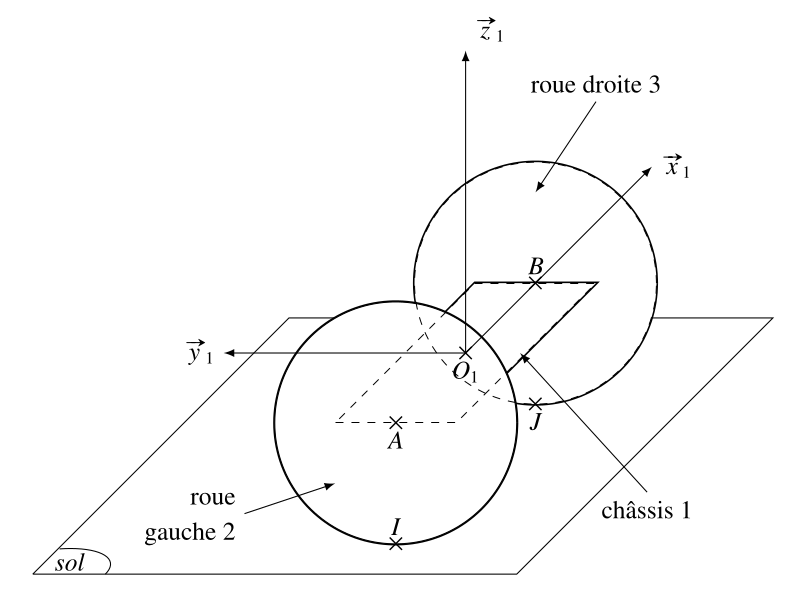
\includegraphics[width=\linewidth]{img/fig06}
 \caption{\label{fig06}Paramétrage du Hublex en perspective}
 \end{minipage}\hfill
 \begin{minipage}{0.45\linewidth}
 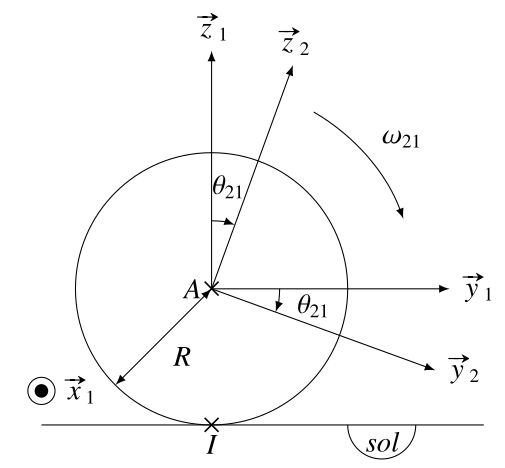
\includegraphics[width=.9\linewidth]{img/fig07}
 \caption{\label{fig07}Paramétrage de la roue gauche 2}
 \end{minipage}
\end{figure}

\begin{figure}[ht!]
 \begin{center}
 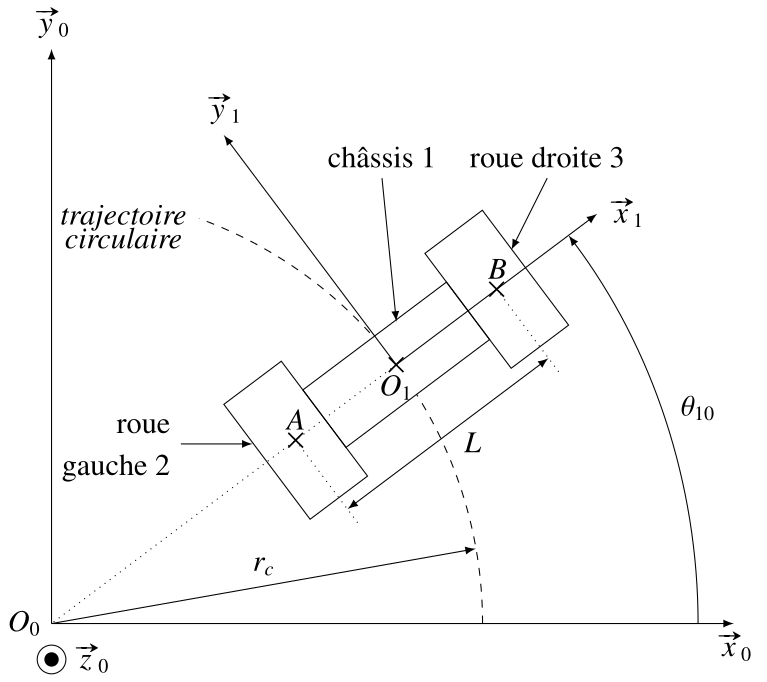
\includegraphics[width=.5\linewidth]{img/fig08}
 \caption{\label{fig08}Hublex dans une trajectoire circulaire}
 \end{center}
\end{figure}

\begin{figure}[ht!]
 \begin{center}
 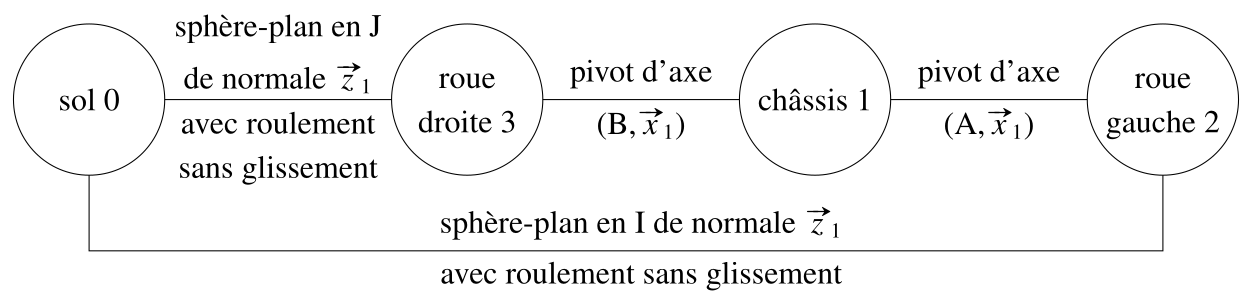
\includegraphics[width=.85\linewidth]{img/fig09}
 \caption{\label{fig09}Graphe des liaisons}
 \end{center}
\end{figure}

\subsection{Génération de la consigne de taux de rotation}

La vitesse angulaire à imposer aux moteurs dépend donc de deux consignes fournies par le pilote : une consigne de vitesse $V_c$ générée à partir de l'inclinaison du gyropode et une consigne de taux de rotation $\omega_{10c}$ obtenue en tournant la poignée d'un angle $\delta$ au niveau du manche et mesurée par un potentiomètre angulaire numérique.

Pour recueillir la consigne de virage imposée par le pilote, on utilise un potentiomètre numérique ayant $360^{\circ}$ d'amplitude et fournissant une image de la position angulaire de la poignée sous forme d'un mot binaire de $10 bits$ soit $2^{10}$ incréments ($inc$). La rotation de la poignée est mécaniquement bloquée entre les angles $-45^{\circ}$ et $+45^{\circ}$. L'absence de rotation de la poignée (i.e. $\delta=0^{\circ}$) correspond au mot binaire valant 0 qui représente une consigne de trajectoire rectiligne.

\question{Donner la résolution de ce capteur, c'est-à-dire sa précision angulaire en $^{\circ}.inc^{-1}$.}

\question{Donner le nombre d'incréments effectivement mesurables avec la poignée du Hublex, ainsi que
la plage des valeurs centrée autour de 0.}

Pour des raisons de sécurité et de confort, l'exigence \og 1.4.3 \fg\ impose que l'accélération centrifuge dans un virage soit limitée à $a_{f\ max}=0.5\cdot g$, avec $g=9.81m\cdot s^{-2}$ l'accélération de la pesanteur. Cette accélération centrifuge est définie par le rapport $a_f=\dfrac{V^2}{r_c}$.

\question{Établir la relation entre $a_f$, $V$ et $\omega_{10}$. En déduire la valeur maximale $\omega_{10\ max}$ du taux de rotation admissible satisfaisant l'exigence \og 1.4 \fg\ et ses sous-exigences.}

On considère que la valeur $\omega_{10\ max}$ est associée à un rayon de courbure minimal atteint lorsque $\delta=45^{\circ}$ (poignée tournée au maximum) et que le rayon de courbure maximal est obtenu pour $\delta=0^{\circ}$ (poignée au centre). En choisissant un modèle de proportionnalité inverse, on obtient les deux relations suivantes reliant les consignes de vitesse des deux moteurs à la consigne fournie par le pilote en se penchant (liée à $V$) et à la consigne issue de la poignée (liée à $\delta$) :

\begin{eqnarray}
V-L\cdot\dfrac{g\cdot\delta}{V\cdot\pi}=-R\cdot k\cdot\omega_{41},\\
V+L\cdot\dfrac{g\cdot\delta}{V\cdot\pi}=-R\cdot k\cdot\omega_{51}.
\end{eqnarray}

\question{Compléter le schéma bloc du document réponse, représentant la génération des commandes des deux moteurs à partir des consignes données par le pilote permettant de respecter l'exigence \og 1.1.1 \fg\ notamment.}

\section{Étude de l'asservissement en intensité des moteurs}

\paragraph{Objectif :} modéliser la chaîne d'asservissement en intensité du moteur afin de déterminer les paramètres du correcteur permettant de respecter l'exigence \og 1.7.1.1 \fg\ et ses sous-exigences.

\paragraph{Modélisation du moteur}

Le moteur brushless associé à son électronique de commande peut se modéliser par les équations d'une machine à courant continu. Les paramètres du modèle associé sont une résistance interne $R$ (en $\Omega$), une inductance $L$ (en $H$) et un coefficient de couplage $K_e$ (en $V\cdot s\cdot rad^{-1}$ ou en $N\cdot m\cdot A^{-1}$).

On notera $i(t)$ l'intensité traversant l'induit (en $A$), $u(t)$ la tension aux bornes de l'induit (en $V$), $e(t)$ la force contre-électromotrice (en $V$), $C_m(t)$ le couple utile délivré par l'action du stator du moteur sur l'arbre (en $N\cdot m$) et $\omega_m(t)$ la vitesse de rotation de l'arbre moteur (en $rad\cdot s^{-1}$). Dans le domaine de Laplace, ces grandeurs seront notées respectivement $I(p)$, $U(p)$, $E(p)$, $C_m(p)$ et $\Omega_m(p)$, avec $p$ la variable dans le domaine de Laplace. On se place dans les conditions d'Heaviside.

On notera $J_{eq}$ l'inertie équivalente des masses mobiles mises en jeu ramenée sur l'arbre moteur. On
modélisera les différents frottements par un frottement visqueux générant un couple résistant, rapporté
à l'arbre moteur, proportionnel à la vitesse de rotation de l'arbre moteur et de coefficient $f\ (f>0)$.

On rappelle les équations caractéristiques associées :\\
\begin{minipage}{.45\linewidth}
\begin{eqnarray}
u(t)=e(t)+R\cdot i(t)+L\cdot \dfrac{di(t)}{dt}\\
e(t)=K_e\cdot\omega_m(t)
\end{eqnarray}
\end{minipage}\hfill
\begin{minipage}{.45\linewidth}
\begin{eqnarray}
C_m(t)=K_e\cdot i(t)\\
J_{eq}\dfrac{d\omega_m(t)}{dt}=C_m(t)-f\cdot \omega_m(t)
\end{eqnarray}
\end{minipage}

\question{Donner, dans le domaine de Laplace, les 4 équations caractéristiques associées au modèle de
machines à courant continu.}

\question{Compléter alors le schéma bloc du moteur du document réponse. On précisera la grandeur associée à chaque lien.}

\question{Donner l'expression de la fonction de transfert $H_m(p)=\dfrac{I(p)}{U(p)}$.
La mettre sous la forme canonique suivante : $H_m(p)=K_m\cdot \dfrac{1+\tau_m\cdot p}{1+\dfrac{2\cdot z_m}{\omega_{0m}}\cdot p+\dfrac{1}{\omega^2_{0m}}\cdot p^2}$}

\paragraph{Asservissement du moteur en intensité}

L'architecture retenue pour contrôler le couple moteur est un asservissement en intensité, image du
couple moteur (voir équation (5)). Le schéma bloc est représenté figure \ref{fig10}. Un convertisseur $IU$
fournit au calculateur une tension $u_{ic}(t)$ image de l'intensité de consigne $i_c(t)$, proportionnelle à cette dernière de coefficient $K_{IU}$. De même, l'intensité réelle $i(t)$, mesurée par un capteur d'intensité de coefficient $K_{capt}$, a pour image $u_{im}(t)$. L'écart, noté $\varepsilon(t)=u_{ic}(t)- u_{im}(t)$, est traité par le correcteur de fonction de transfert $C(p)$, qui impose la tension $u(t)$ aux bornes du moteur.

On note $I_c(p)$, $U_{ic}(p)$, $U_{im}(p)$, $\varepsilon(p)$ les transformées de Laplace respectives de $i_c(t)$, $u_{ic}(t)$, $u_{im}(t)$ et $\varepsilon(t)$.

On donne la fonction de transfert du moteur : $H_m(p)=K_m\cdot \dfrac{1+\tau_m\cdot p}{1+\dfrac{2\cdot z_m}{\omega_{0m}}\cdot p+\dfrac{1}{\omega^2_{0m}}\cdot p^2}$.

\begin{figure}[ht!]
 \begin{center}
 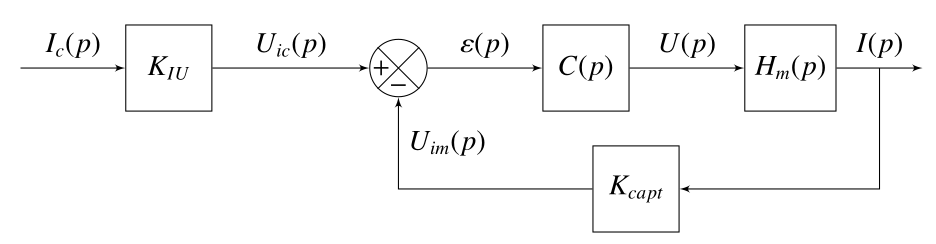
\includegraphics[width=.8\linewidth]{img/fig10}
 \caption{\label{fig10}Schéma bloc de l'asservissement en intensité}
 \end{center}
\end{figure}

\question{Préciser, en justifiant, quelle valeur donner à $K_{IU}$, caractéristique du convertisseur IU.}

On prend, dans un premier temps, un correcteur purement proportionnel : $C(p)=K_p$.

On en déduit la fonction de transfert $H_I(p)=\dfrac{I(p)}{I_c(p)}$:

$H_I(p)=\dfrac{K'}{1+K'}\cdot \dfrac{1+\tau_m\cdot p}{1+\dfrac{\dfrac{2\cdot z_m}{\omega_{0m}}+K'\tau_m}{1+K'}\cdot p+\dfrac{1}{\omega^2_{0m}(1+K')}\cdot p^2}$, avec $K'=K_{iu}\cdot K_p\cdot K_m$.

\question{Calculer l'expression littérale de l'erreur en régime permanent notée $\mu_s$, pour une entrée indicielle (i.e. $I_c(p)$ est un échelon unitaire), en fonction de $K_{iu}$, $K_p$ et $K_m$.}

\question{Conclure, lorsque cela est possible, quant au respect des sous-exigences de l'exigence
\og 1.7.1.1 \fg\ avec ce type de correcteur.}

\newpage

La figure \ref{fig11} présente les diagrammes de Bode en boucle ouverte de l'asservissement étudié, en
prenant $K_p=10$.

\begin{figure}[ht!]
 \begin{center}
 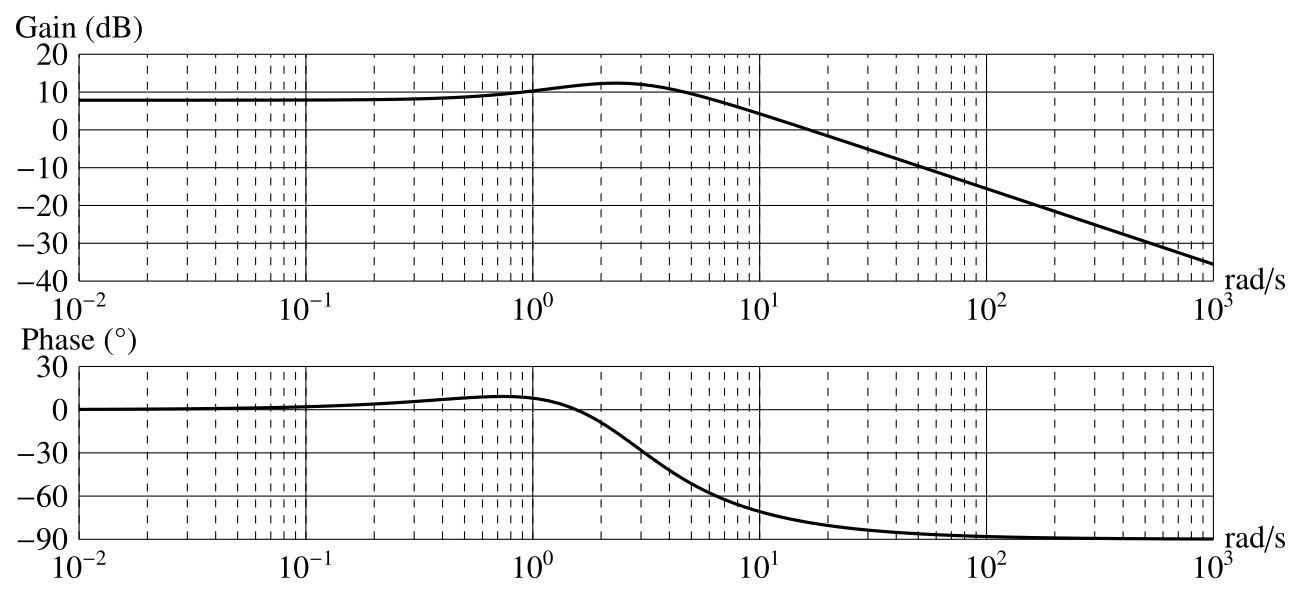
\includegraphics[width=.8\linewidth]{img/fig11}
 \caption{\label{fig11}Diagrammes de Bode en boucle ouverte pour $K_p=10$}
 \end{center}
\end{figure}

Dans un deuxième temps, il est décidé d'utiliser un correcteur de type proportionnel intégral. Sa
fonction de transfert est notée : $C(p)=K_p+\dfrac{K_i}{p}$.

\question{Préciser l'influence de ce correcteur sur les performances du système. Justifier le choix de ce
type de correcteur dans le cas étudié.}

~\

On souhaite régler le correcteur afin de respecter les performances de précision et de stabilité.

\question{Compléter le tableau de variations du Gain (dB) et de la Phase ($^{\circ}$). Tracer sur le document réponse, les diagrammes de Bode asymptotique du correcteur pour $K_p=10$ et $K_i=1000$. On précisera les valeurs numériques associées aux valeurs caractéristiques.}

~\

Pour la suite, on va s'intéresser aux trois exigences suivantes:
\begin{itemize}
 \item \og 1.7.1.1.3\ \fg : Pour $\omega=100rad\cdot s^{-1}$, le gain en db doit être supérieur à 0db,
 \item \og 1.7.1.1.4\ \fg : A la pulsation pour laquelle le gain vaut 0dB, la phase doit être supérieure à $-180+70=-110^{\circ}$,
 \item \og 1.6.1.1\ \fg : qui ne nécessite pas d'explication.
\end{itemize}

\question{Vérifier les exigences (parmi les 3 précédentes) qu'il est possible de vérifier pour la correction proportionnelle (figure \ref{fig11}). Proposer une modification de la valeur de $K_p$ si besoin pour valider ces exigences.}

~\

Avec le réglage précédent, on obtient les diagrammes de Bode en boucle ouverte (figure \ref{fig12}) et les
réponses temporelles (figure \ref{fig13}), pour un échelon d'intensité $i_c(t)$ de $2A$.

\question{Vérifier les exigences (parmi les 3 précédentes) qu'il est possible de vérifier pour le réglage du correcteur Pi (figures \ref{fig12} et \ref{fig13}).}

~\

Le correcteur reste inchangé. Afin de palier le problème identifié précédemment, on apporte une
dernière évolution au sein du calculateur. Cela permet de respecter les exigences de l'asservissement.

La figure \ref{fig14} présente les réponses temporelles du système pour un échelon d'intensité $i_c(t)$ de $2A$.

\question{Préciser quelle ultime modification a apporté le constructeur afin de respecter les exigences de
l'asservissement.}

\begin{figure}[ht!]
 \begin{center}
 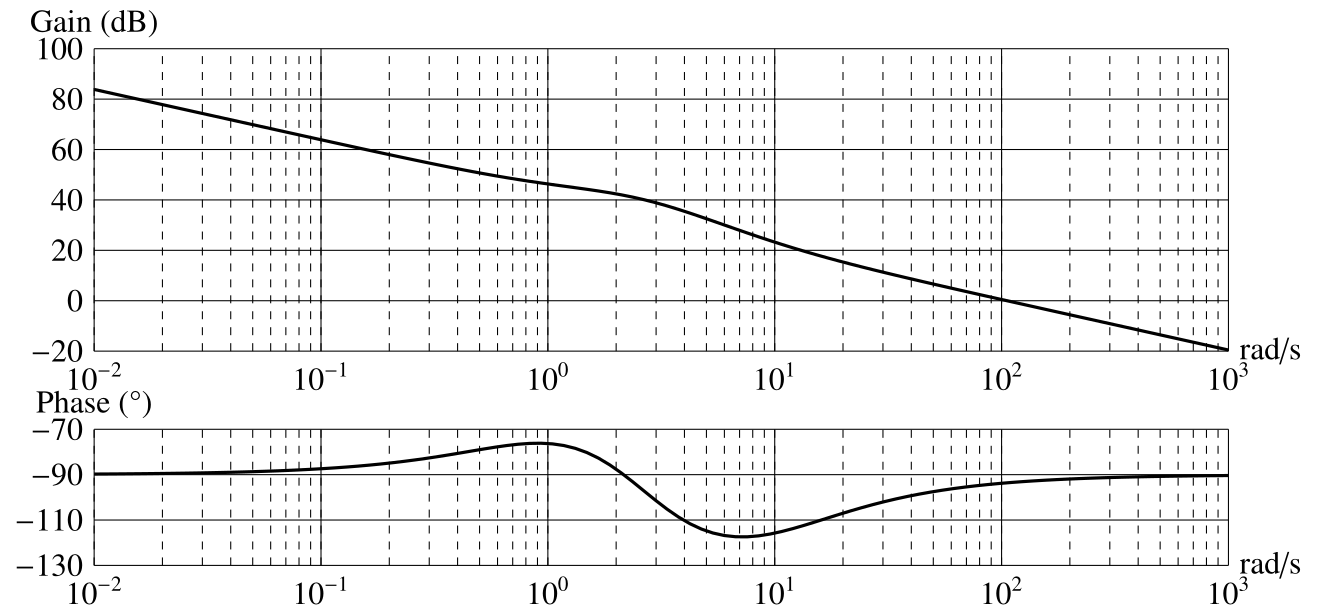
\includegraphics[width=.8\linewidth]{img/fig12}
 \caption{\label{fig12}Diagrammes de Bode en boucle ouverte avec réglage du correcteur PI effectué}
 \end{center}
\end{figure}

\begin{figure}[ht!]
 \begin{minipage}{0.45\linewidth}
 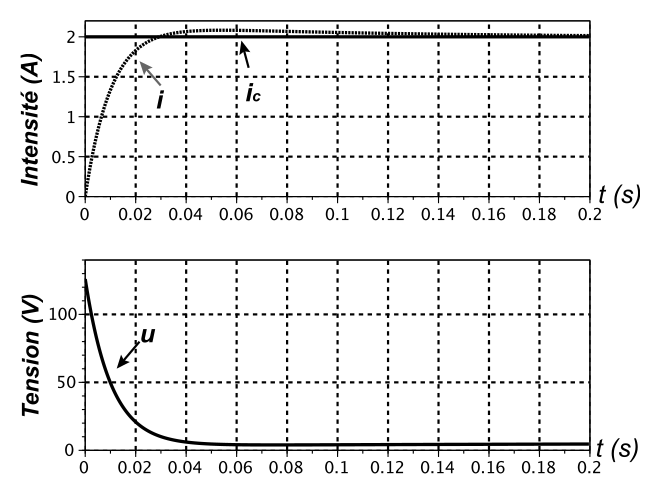
\includegraphics[width=\linewidth]{img/fig13}
 \caption{\label{fig13}Réponses temporelles avec réglage du correcteur PI effectué}
 \end{minipage}\hfill
 \begin{minipage}{0.45\linewidth}
 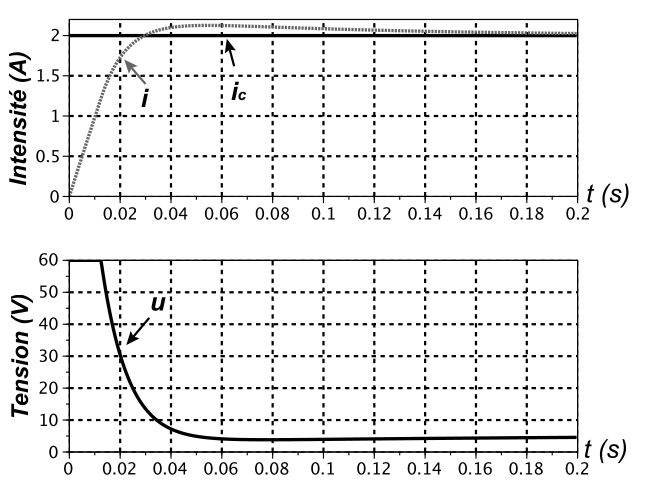
\includegraphics[width=\linewidth]{img/fig14}
 \caption{\label{fig14}Réponses temporelles du système finalement implanté}
 \end{minipage}
\end{figure}

\newpage

\section{Gestion du parc de Hublex}

\paragraph{Objectif:} Analyser et concevoir des fonctions informatiques nécessaires à un programme permettant la gestion d'une flotte de Hublex.

Le Hublex a été conçu pour être commercialisé sous forme d'une flotte partagée. Dans ce cadre, deux applications ont été développées : la première permet de réaliser des réservations en ligne (on parlera de phase de réservation) et la seconde permet d'attribuer un Hublex précis à une réservation (on parlera de phase de planification).

On s'intéresse tout d'abord à la base de données associée à l'application permettant de réserver un
Hublex. Elle contient l'ensemble des informations liées aux réservations et aux utilisateurs.

Les heures de début et de fin de réservations sont toujours des heures pleines (par exemple : 13:00, 14:00, 15:00 ...) et les opérateurs usuels (somme, soustraction, comparaison,...) sont
autorisés sur les données au format time.

Chaque soir est extrait de la base de données l'ensemble des réservations pour le lendemain. Chaque
réservation est stockée sous forme d'une liste contenant trois éléments :
\begin{itemize}
 \item un identifiant,
 \item une heure de début de réservation,
 \item une durée.
\end{itemize}

Ainsi la liste [5,14,3] représente la réservation numéro 5, commençant à 14 h et d'une durée de 3 heures. 

L'ensemble des réservations d'une journée est stocké dans la liste nommée extraction contenant une ou plusieurs réservations (on fera l'hypothèse qu'il y a toujours au moins une réservation).

On pourra prendre l'exemple suivant :
\begin{center}
\texttt{extraction = [[1,9,3],[2,18,1],[3,11,4],[4,17,2],[5,14,3],[6,12,2],[7,9,8]]}
\end{center}

Une flotte de \verb?n? Hublex (\verb?n? un entier non nul, on considérera \verb?n = 3? pour exemple) étant disponible, une application simple a été développée afin de répartir les réservations sur les \verb?n? Hublex disponibles, avec comme contrainte de répartir la charge (c'est-à-dire la durée de réservation) au mieux entre les différents Hublex.

Avant de procéder à cette affectation, le choix a été fait de trier les réservations en fonction de leur
durée, les réservations les plus longues représentant les charges les plus importantes et devant donc
être affectées en premier. Pour cela la fonction \verb?tri_reservations? est utilisée.

Ainsi, l'instruction \verb?tri_reservations(extraction)? qui utilise cette fonction modifie la liste de départ pour obtenir une nouvelle version de la liste extraction :
\begin{center}
\texttt{extraction = [[7,9,8],[3,11,4],[1,9,3],[5,14,3],[4,17,2],[6,12,2],[2,18,1]]}
\end{center}

\question{Écrire en langage Python une fonction \texttt{conflit2(R1,R2)} prenant en argument deux listes représentant deux réservations \verb?R1? et \verb?R2? et renvoyant un booléen indiquant si les deux réservations sont en conflit potentiel, c'est-à-dire que l'intersection de leurs deux créneaux horaires est non vide. Par exemple \verb?conflit2([5,14,3],[7,9,8])? renvoie \verb?True? (la réservation numéro \textbf{7} se termine à 17h, après le début de la réservation numéro \textbf{5}) et \verb?conflit2([5,14,3],[6,12,2])? renvoie \verb?False? (la réservation numéro \textbf{6} se termine à 14h, soit avant ou au début de la réservation numéro \textbf{5}).}

\question{En exploitant la fonction \texttt{conflit2}, écrire en langage Python une fonction \texttt{sans\_conflitL(R1,L)} prenant deux arguments : une liste \texttt{R1} représentant une réservation et une liste \texttt{L} contenant plusieurs listes (liste de listes) représentant des réservations. Cette fonction devra renvoyer un booléen indiquant si la réservation \texttt{R1} est en conflit avec au moins l'une des réservations contenues dans \texttt{L}.

Par exemple \texttt{sans\_conflitL([5,14,3],[[4,17,2],[6,12,2],[2,18,1]])} renvoie \texttt{True} et \texttt{sans\_conflitL([5,14,3],[[7,9,8],[3,11,4],[1,9,3]])} renvoie \verb?False?.}

\question{Écrire en langage Python une fonction \texttt{ind\_max} prenant en argument une liste et renvoyant l'indice de position de la valeur maximale.

Par exemple, \texttt{ind\_max([3,5,8,6,7])} renvoie \verb?2? et \texttt{ind\_max([5,9,4,9])} renvoie \verb?1?. \textbf{On n'utilisera pas les fonctions/méthodes définies dans Python comme la fonction max ou la méthode index propre aux listes.}}

\section{Annexe}

\begin{figure}[ht!]
 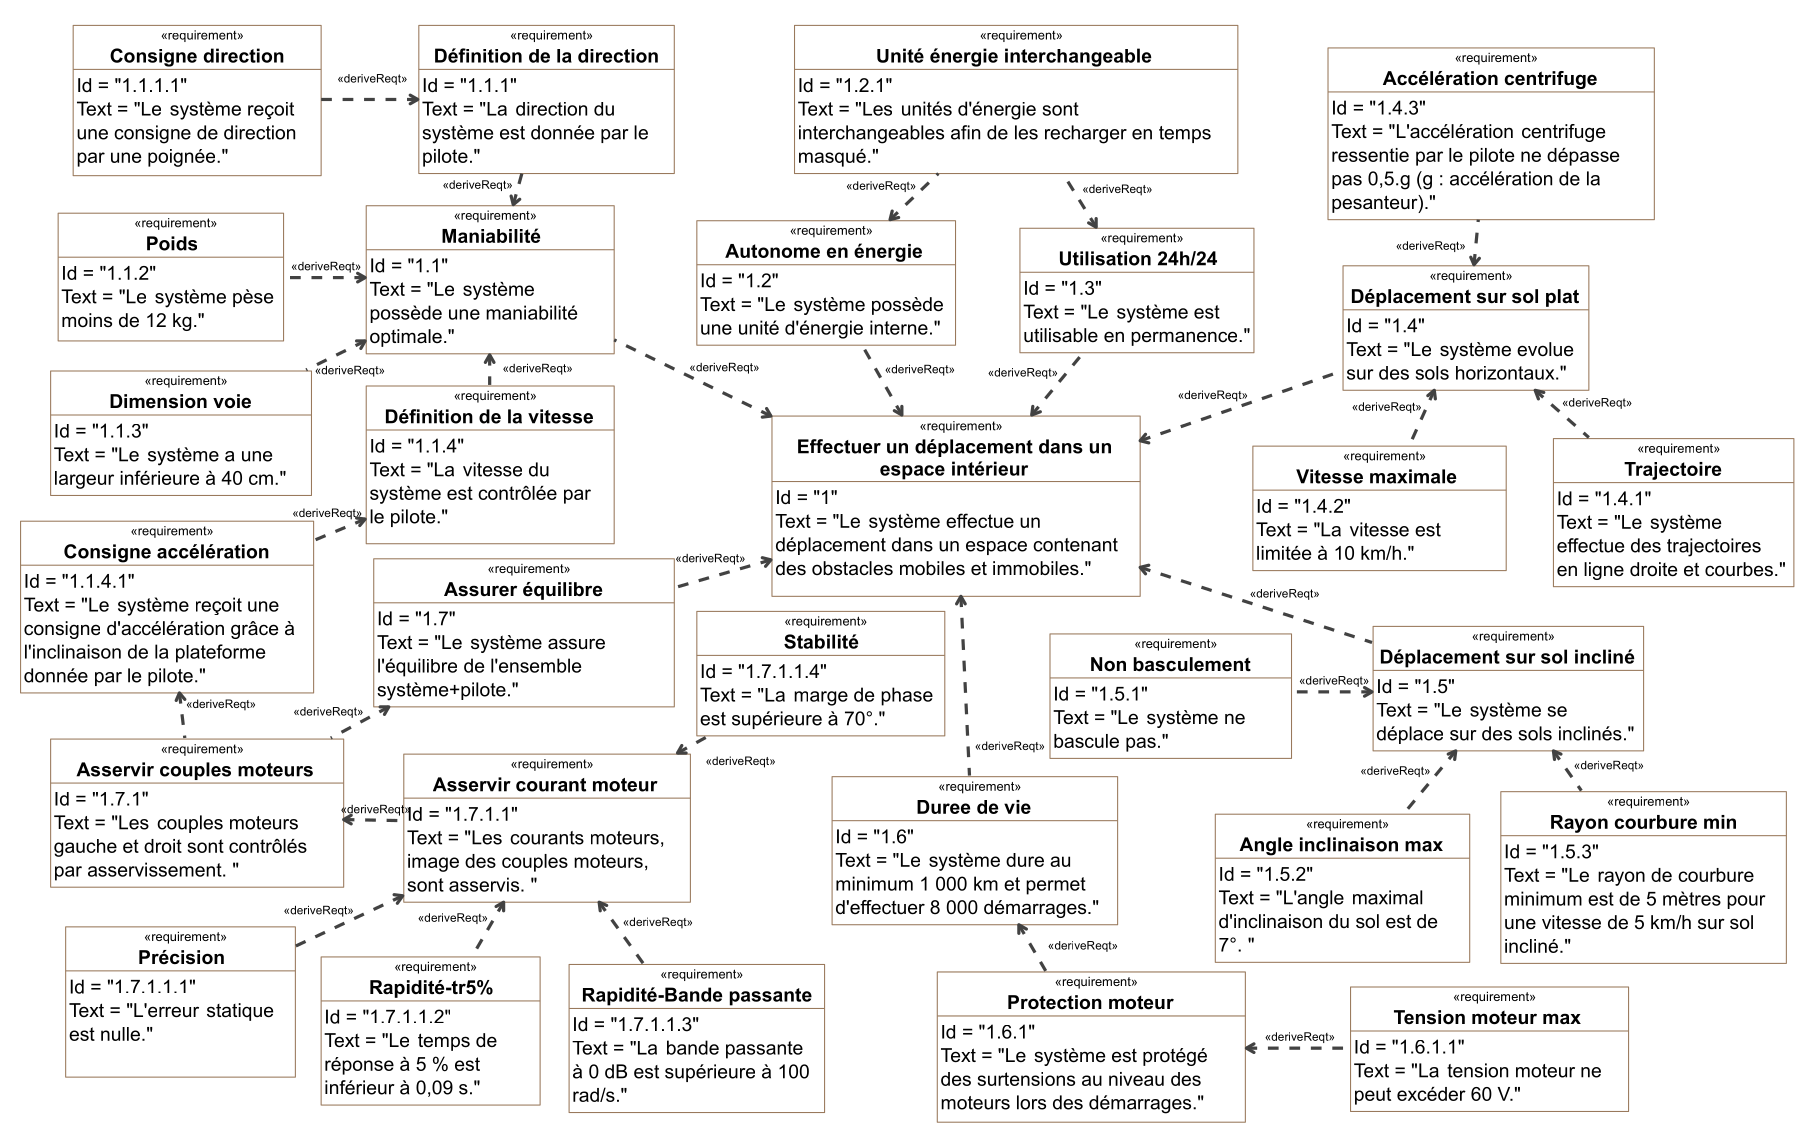
\includegraphics[width=\linewidth]{img/fig16}
 \caption{\label{fig16}Diagramme des exigences}
\end{figure}

\finsujet

\reponse{0}{
\begin{center}
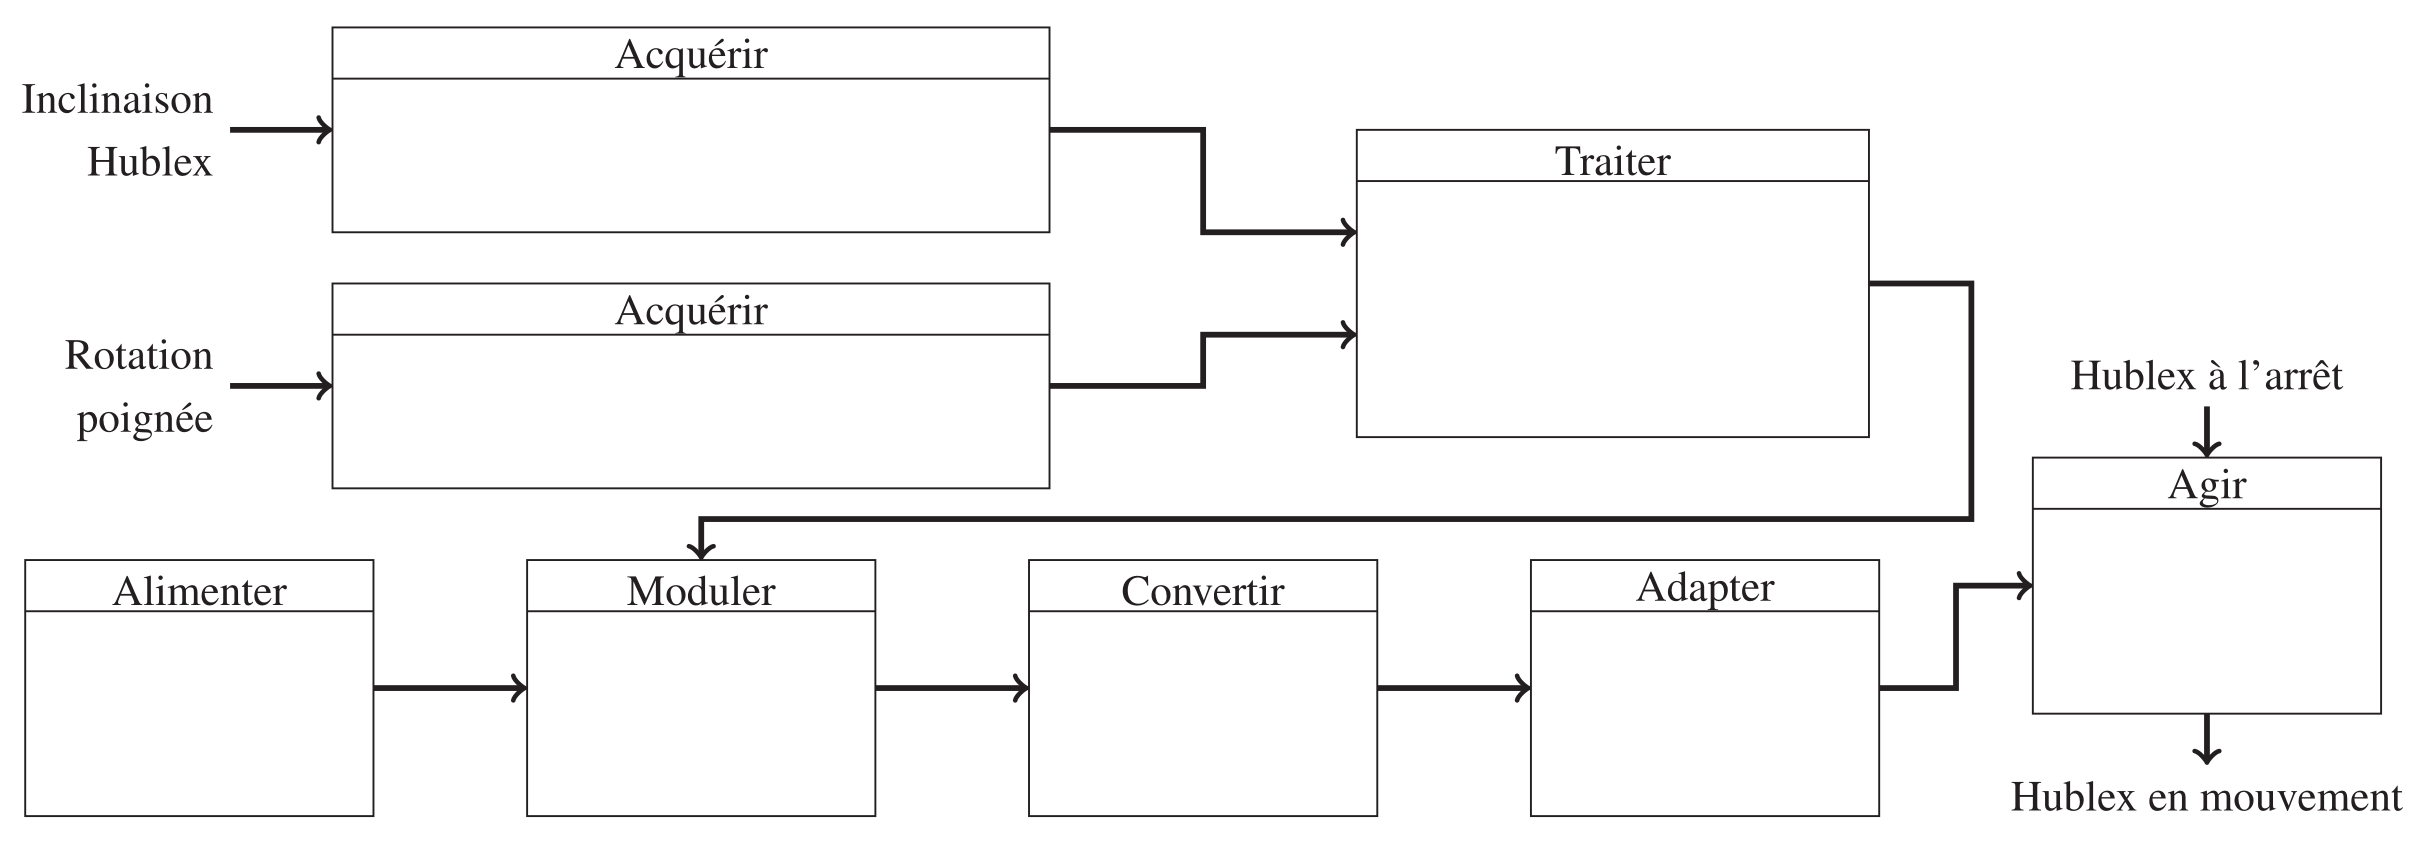
\includegraphics[width=\linewidth]{img/DR01}
\end{center}
}
{
\begin{center}
\def\svgwidth{\linewidth}
\input{img/DR01_cor.pdf_tex}
\end{center}
}

\reponse{4}{}{$\left[\dfrac{d\overrightarrow{O_0O_1}}{dt}\right]_{R_0}=r_c\cdot\left[\dfrac{d\vec{x_1}}{dt}\right]_{R_0}=r_c\cdot\overrightarrow{\Omega_{1/0}}\wedge\vec{x_1}=r_c\cdot\omega_{10}\cdot\vec{y_1}=V\cdot\vec{y_1}$, ainsi, $V=r_c\cdot\omega_{10}$}

\reponse{4}{}{$\overrightarrow{V_{A\in 2/0}}=\overrightarrow{V_{I\in 2/0}}+\overrightarrow{AI}\wedge\overrightarrow{\Omega_{2/0}}=-R\cdot\vec{z_1}\wedge\left(\omega_{21}\cdot\vec{x_1}+\omega_{10}\cdot\vec{z_1}\right)=-R\cdot\omega_{21}\cdot\vec{y_1}=\overrightarrow{V_{A\in 2/1}}+\overrightarrow{V_{A\in 1/0}}=\left(r_c-\dfrac{L}{2}\right)\cdot\omega_{10}\cdot\vec{y_1}$

Donc, $V-\dfrac{L}{2}\cdot\omega_{10}+R\cdot\omega_{21}=0$}

\reponse{3}{}{$V-\dfrac{L}{2}\cdot\omega_{10}+R\cdot k\cdot\omega_{41}=0$ donc $\omega_{41}=\dfrac{\dfrac{L}{2}\cdot \omega_{10}- V}{R\cdot k}$}

\reponse{5}{}{$\overrightarrow{V_{J\in 3/0}}=\vec{0}\ \Rightarrow\ 
\overrightarrow{V_{B\in 3/0}}=\overrightarrow{V_{J\in 3/0}}+\overrightarrow{BJ}\wedge\overrightarrow{\Omega_{3/0}}=-R\cdot \omega_{31}\cdot\vec{y_1}$

$\overrightarrow{V_{B\in 3/0}}=\overrightarrow{V_{B\in 3/1}}+\overrightarrow{V_{B\in 1/0}}=\left(r_c+\dfrac{L}{2}\right)\cdot\omega_{10}\cdot\vec{y_1}$

Donc $-R\cdot\omega_{31}=\left(r_c+\dfrac{L}{2}\right)\cdot\omega_{10}=V+\dfrac{L}{2}\cdot\omega_{10}$

$-R\cdot k\cdot\omega_{51}=V+\dfrac{L}{2}\cdot\omega_{10}$

$\omega_{51}=-\dfrac{V+\dfrac{L}{2}\cdot\omega_{10}}{R\cdot k\cdot}$}

\reponse{3}{}{La résolution est de $\dfrac{360^{\circ}}{2^{10}inc}=0.35^{\circ}.inc^{-1}$}

\reponse{3}{}{$-45^{\circ}\leq 9 \leq 45^{\circ}$ donc $\dfrac{90^{\circ}\cdot 1024}{360^{\circ}}=256valeurs$, soit de $-128$ à $128$.}

\reponse{4}{}{$\alpha_f=\dfrac{V^2}{r_c}=\dfrac{V^2}{\dfrac{V}{\omega_{10}}}=V\cdot \omega_{10}$

Donc $\omega_{10\ max}=\dfrac{\alpha_{f\ max}}{V_{max}}=\dfrac{0,5\cdot 9,81}{\dfrac{10\cdot 10^3}{3600}}=\dfrac{3,6\cdot 0,5\cdot 9,81}{10}=1,75rad\cdot s^{-1}$.}

\reponse{0}{
\begin{center}
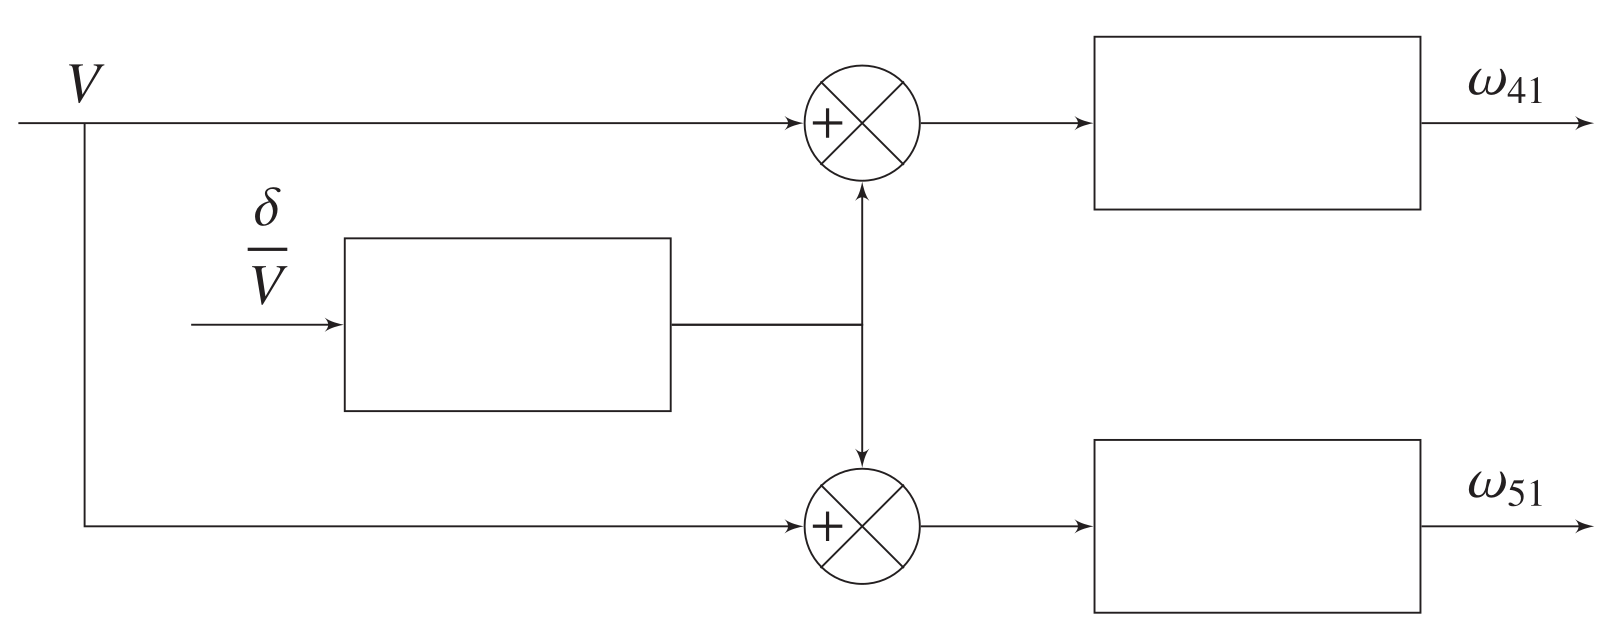
\includegraphics[width=0.6\linewidth]{img/DR02}
\end{center}
}
{
\begin{center}
\def\svgwidth{0.7\linewidth}
\input{img/DR02_cor.pdf_tex}
\end{center}
}

\reponse{3}{}{
$U(p)=E(p)+R\cdot I(p)+L\cdot p\cdot I(p)$

$E(p)=K_e\cdot\Omega_m(p)$

$C_m(p)=K_e\cdot I(p)$

$J_{eq}\cdot p\cdot \Omega_m(p)=C_m(p)-f\cdot \Omega_m(p)$}

\reponse{0}{
\begin{center}
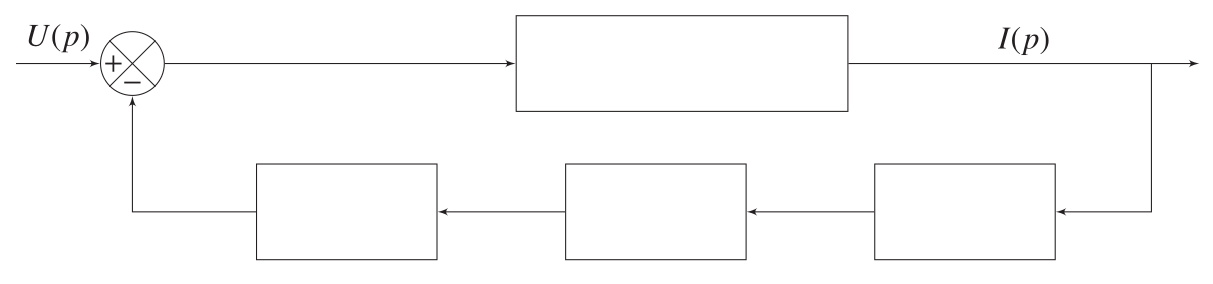
\includegraphics[width=\linewidth]{img/DR03}
\end{center}
}
{
\begin{center}
\def\svgwidth{\linewidth}
\input{img/DR03_cor.pdf_tex}
\end{center}
}

\reponse{5}{}{
$H_m(p)=\dfrac{1}{R+L\cdot p}\cdot \dfrac{1}{1+\dfrac{K_e^2}{(R+L\cdot p)\cdot (f+J_{eq}\cdot p)}}=
\dfrac{f+J_{eq}\cdot p}{(R+L\cdot p)\cdot (f+J_{eq}\cdot p)+K_e^2}=
\dfrac{f+J_{eq}\cdot p}{(K_e^2+R\cdot f)+(R\cdot J_{eq}+L\cdot f)\cdot p+(L\cdot J_{eq})\cdot p^2}$

$H_m(p)=K_m\cdot\dfrac{1+\tau_m\cdot p}{1+\dfrac{2\cdot z_m}{\omega_{0m}}\cdot p+\dfrac{1}{\omega_{0m}}\cdot p^2}$

Avec:
\begin{itemize}
 \item $K_m=\dfrac{f}{K_e^2+R\cdot f}$
 \item $\tau_m=\dfrac{J_{eq}}{f}$
 \item $z_m=\dfrac{R\cdot J_{eq}+L\cdot f}{2\sqrt{L\cdot J_{eq}\cdot(K_e^2+R\cdot f)}}$,
 \item $\omega_{0m}=\sqrt{\dfrac{K_e^2+R\cdot f}{L\cdot J_{eq}}}$.
\end{itemize}
}

\reponse{5}{}{
On veut $\varepsilon(p)=0$ quand $I(p)=I_c(p)$ quelle que soit la consigne $I_c(p)$ avec $\varepsilon(p)=K_{IU}\cdot I_c(p)-K_{capt}\cdot I(p)$.

Soit $0=I_c(p)\cdot (K_{IU}-K_{capt})$
On doit donc régler $K_{IU}=K_{capt}$}

\reponse{7}{}{
D'après le théorème de la valeur finale $\mu_s=\lim\limits_{t\rightarrow \infty}\varepsilon(t)=\lim\limits_{p\rightarrow 0}p\cdot\varepsilon(p)$.

Avec $I_c(p)=\dfrac{1}{p}$, $\varepsilon(p)=I_c(p)\cdot \left(1-\dfrac{K'}{1+K'}\cdot\dfrac{1+\tau_m\cdot p}{1+\dfrac{\dfrac{2\cdot z_m}{\omega_{0m}}+K'\cdot \tau_m}{1+K'}\cdot p+\dfrac{1}{\omega_{0m}^2\cdot (1+K')}\cdot p^2}\right)$

Donc $\mu_s=\dfrac{1}{1+K'}=\dfrac{1}{1+K_{iu}\cdot K_p\cdot K_m}$}

\reponse{4}{}{$\mu_s\neq0$ donc l’exigence 1.7.1.1.1 n’est pas satisfaite}

\reponse{4}{}{Le correcteur proportionnel intégral utilisé permet d’améliorer la précision pour satisfaire à l’exigence \og 1.7.1.1.1\ \fg.}

\reponse{5}{
\begin{tabular}{|p{0.1\linewidth}|p{0.4\linewidth}|p{0.4\linewidth}|}
\hline
$\omega$ & 0\hfill $\dfrac{K_i}{K_p}$ & $\dfrac{K_i}{K_p}$ \hfill $+\infty$ \\
\hline
Gain $(db)$ &  & \\[50pt]
\hline
Phase $(^{\circ})$ &  & \\[50pt]
\hline
\end{tabular}

\begin{center}
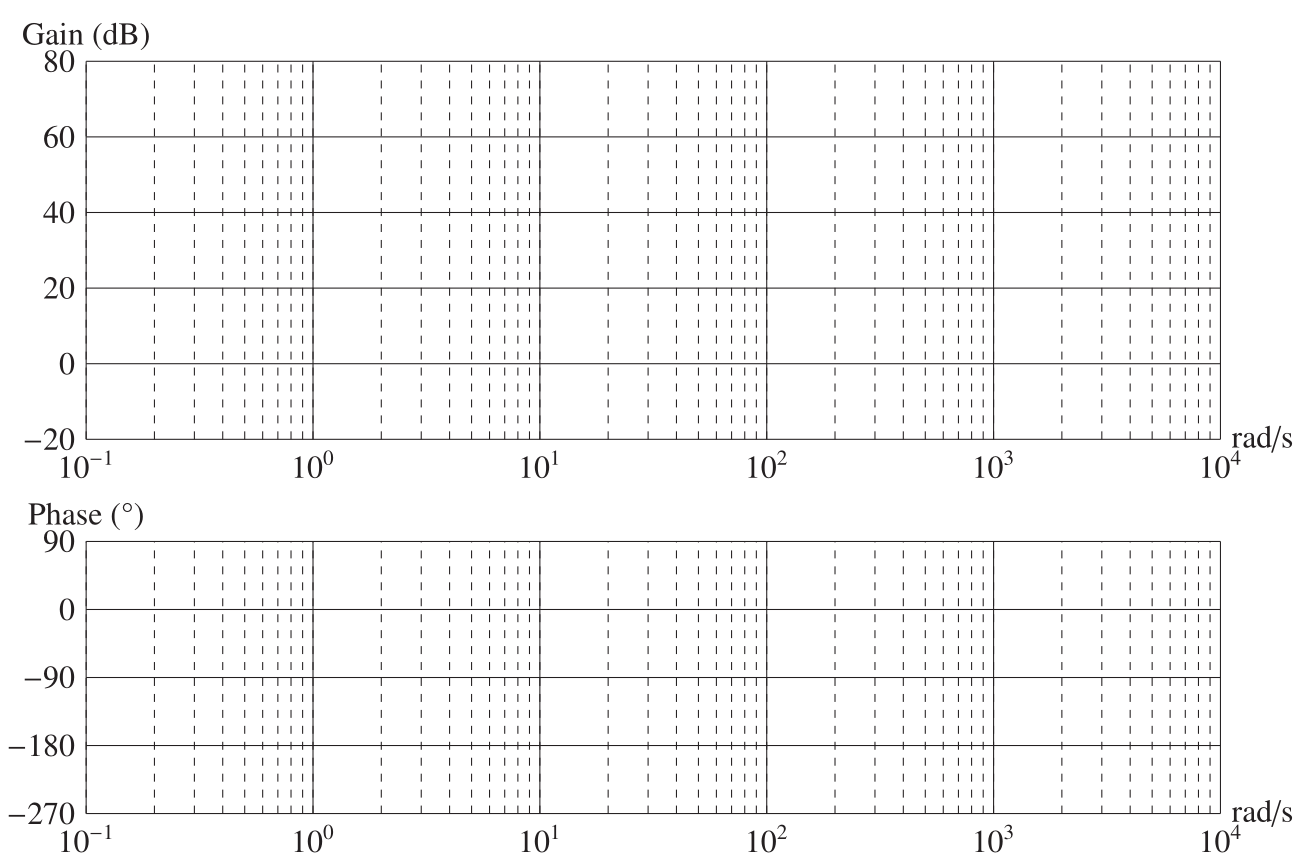
\includegraphics[width=\linewidth]{img/DR04}
\end{center}
}{$C(p)=K_p+\dfrac{K_i}{p}=K_i\cdot \dfrac{1}{p}\cdot \left(\dfrac{K_p}{K_i}\cdot p+1\right)$

\begin{tabular}{|p{0.1\linewidth}|p{0.4\linewidth}|p{0.4\linewidth}|}
\hline
$\omega$ & 0\hfill $\dfrac{K_i}{K_p}$ & $\dfrac{K_i}{K_p}$ \hfill $+\infty$ \\
\hline
Gain $(db)$ & $20\log\left(\dfrac{K_i}{p}\right)=20\log(K_i)-20\log(p)$ Pente de $-20dB/dec$& $20\log(K_p)$ \\
\hline
Phase $(^{\circ})$ & $-90^{\circ}$ & $0^{\circ}$ \\
\hline
\end{tabular}

\begin{center}
\def\svgwidth{\linewidth}
\input{img/DR04_cor.pdf_tex}
\end{center}
}


\reponse{5}{}{
Sur la figure \ref{fig11}, la valeur de déphasage reste supérieure à $-110^{\circ}$ donc l’exigence de stabilité \og 1.7.1.1.4\ \fg est satisfaite indépendamment de la valeur de réglage de $K_p$.

L'exigence \og 1.7.1.1.4\ \fg demande un gain positif pour $\omega=100 rad\cdot s^{-1}$. Sur la figure \ref{fig11}, on relève GdB ($100 rad\cdot s^{-1}=-16dB$ pour $K_p=10$.

Il faut donc multiplier $K_p$ par $10^{\dfrac{16}{20}}\approx 6,31$, soit $K_p=63,1$.}

\reponse{5}{}{
Par lecture, on voit que l’exigence \og 1.7.1.1.3\ \fg est satisfaite.

Sur la figure \ref{fig12}, on relève pour $\omega_{OdB}$ une phase égale à $\approx -85^{\circ}>-110^{\circ}$, l’exigence \og 1.7.1.1.4\ \fg est satisfaite.

Sur la figure \ref{fig13}, on relève un pic de tension au démarrage avec une tension supérieure à $60V$. Ce réglage ne permet pas de satisfaire à l’exigence \og 1.6.1.1\ \fg.
}

\reponse{3}{}{Afin de de satisfaire à l’exigence \og 1.6.1.1\ \fg, le constructeur a ajouté une saturation en tension à $60V$.}

\reponseinfo{7}

\ifprintdr
\fi

\ifprintcor
\begin{minted}[xleftmargin=2em,linenos,firstnumber=30]{python}
def conflit2(R1,R2):
	if R1[1]>= R2[1] and R2[1]+R2[2]>R1[1]:
		return True
	elif R1[1]<R2[1] and R1[1]+R1[2]>R2[1]:
		return True
	else:
	    return False
\end{minted}
\fi

\reponseinfo{7}

\ifprintdr
\fi

\ifprintcor
\begin{minted}[xleftmargin=2em,linenos,firstnumber=30]{python}
def sans_conflitL(R1,L):
	for reservation in L:
		if conflit2(R1,reservation):
			return False
	return True
\end{minted}
\fi

\reponseinfo{7}

\ifprintdr
\fi

\ifprintcor
\begin{minted}[xleftmargin=2em,linenos,firstnumber=30]{python}
def ind_max(liste):
	indice=0
	val_max=liste[indice]
	for i in range(1,len(liste)):
		if liste[i]> val_max:
		indice=i
		val_max =liste[indice]
	return indice
\end{minted}
\fi

\end{document}
